\documentclass[12pt,ngerman]{scrartcl}

\usepackage{tikz}

\begin{document}

Hallo TikZ!

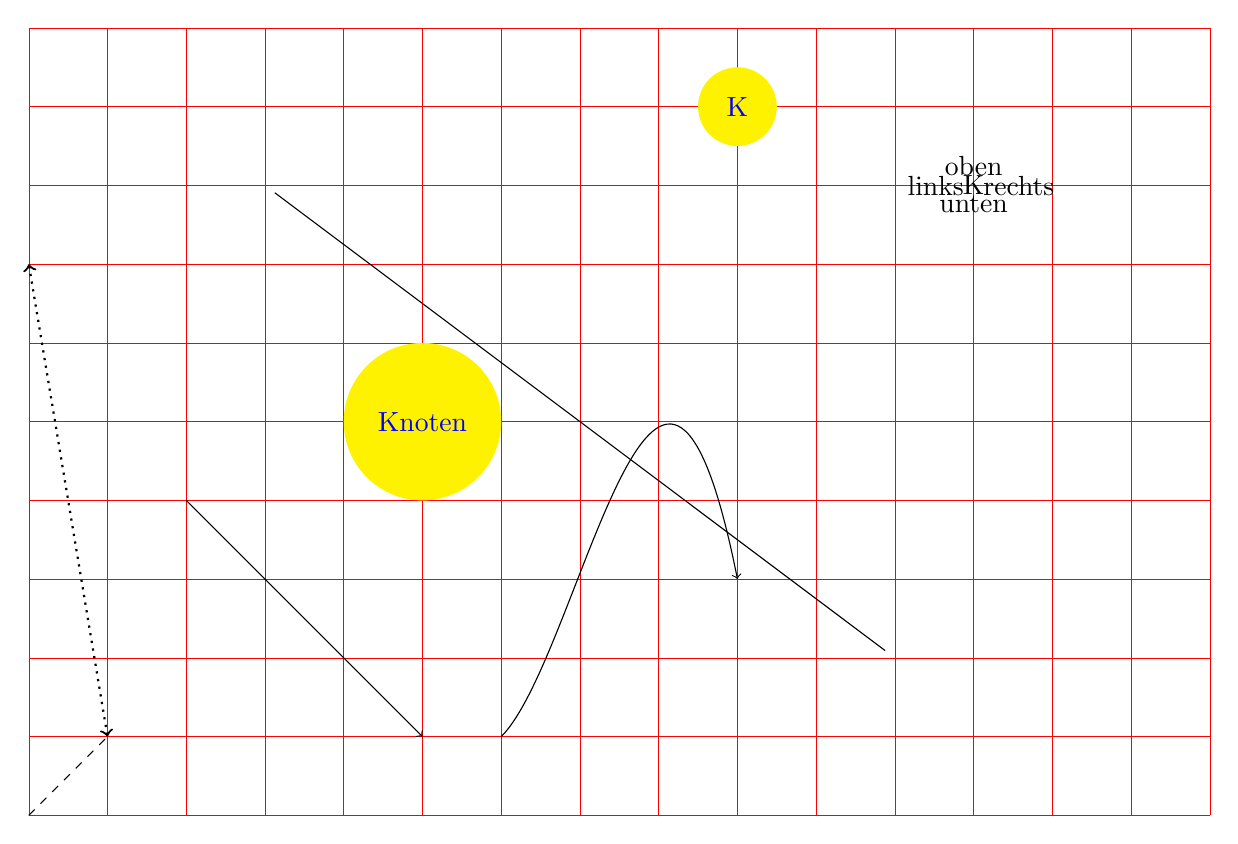
\begin{tikzpicture}[
punkt/.style={circle, minimum size = 2cm, blue,fill=yellow},
kleinpunkt/.style={punkt, minimum size = 1cm},
]
\draw[help lines,red] (0,0) grid (15,10);
\draw[dashed] (0,0) -- (1,1);
\draw[dotted,<->,thick] (1,1) -- (0,7);
\draw[->] (2,4) -- (5,1);

\draw[->] (6,1) .. controls (7,2) and (8,8) .. (9,3);

\node[punkt] at (5,5) {Knoten};

\node[kleinpunkt] at (9,9) {K};

\node (A) at (3,8){};
\node (B) at (11,2){};

\draw (A) -- (B);

\node at (12,8) {K};
\node [below] at (12,8){unten};
\node [above] at (12,8){oben};
\node [left] at (12,8){links};
\node [right] at (12,8){rechts};


\end{tikzpicture}

Hallo TikZ!

\end{document}